%نام و نام خانوادگی:
%شماره دانشجویی: 
\مسئله{پارسر LR(0)}

\پاسخ{
\begin{enumerate}
	\item
	
		\begin{figure}[H]
			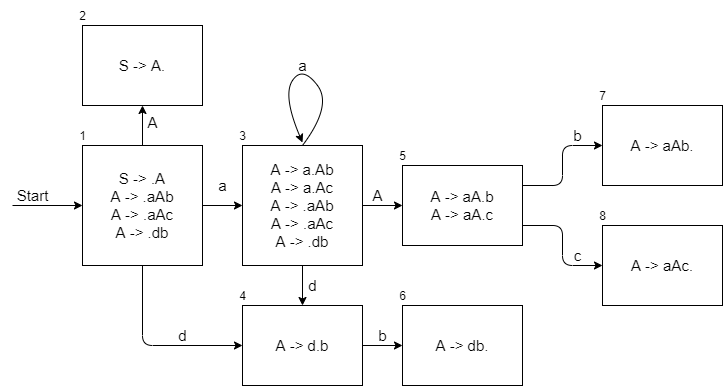
\includegraphics[width=\linewidth]{./commons/Q6.png}
			\label{fig:Q6}
		\end{figure}
		\lr{
		\begin{table}[H]
			\begin{tabular}{c|c|c|c|c|c|c|c|c}
				 & a   & b   & c  & d   & A \\
				\hline
				1 & S3 &      &     & S4 & G2 \\
				2 &acc &acc &acc &acc &acc\\
				3 & S3 &      &      & S4 & G5 \\
				4 &      & S6 &      &      &     \\
				5 &      & S7 & S8 &      &     \\
				6 & R4 & R4 & R4 & R4 & R4 \\
				7 & R2 & R2 & R2 & R2 & R2 \\
				8 & R3 & R3 & R3 & R3 & R3 \\
				\hline
			\end{tabular}
		\end{table}
		}
	\item
ابتدا در حالت 1 قرار داریم.(a|adbc)\\
با خواندن a به حالت 3 میرویم و توکن بعدی را میخوانیم. (aa|dbc)\\
در این حالت نیز، باز با خواندن a به حالت 3 میرویم و توکن بعدی را میخوانیم. (aad|bc)\\
حال با خواندن d به حالت 4 میرویم و توکن بعدی را میخوانیم. (aadb|c)\\
حال با خواندن b به حالت 6 میرویم که در این حالت، reduction داریم به صورت A $\rightarrow$ db پس 2 حالت به عقب میرویم(حالت 3) و db را نیز به A تبدیل میکنیم.(aaA|c)\\
حال در حالت 3 هستیم و با خواندن A به حالت 5 میرویم. توکن بعدی را میخوانیم. (aaAc|)\\
حال با خواندن c به حالت 8 میرویم که در این حالت، reduction داریم به صورت A $\rightarrow$ aAc پس 3 حالت به عقب میرویم(حالت 3) و aAc را نیز به A تبدیل میکنیم. (aA|)\\
حال در حالت 3 هستیم و با خواندن A به حالت 5 میرویم.و همین جا گیر میفتیم.چرا که aA را داریم و دیگر هیچ.\\
پس نمیتوان این رشته را پارس کرد.\\

\end{enumerate}
}